%! Author = Runge
%! Date = 29-12-2023

% Preamble
\documentclass[english,a4paper,compsoc,journal]{IEEEtran}
\overfullrule=10pt
\frenchspacing

% Packages
%! Author = Runge
%! Date = 29-12-2023

% Packages
\RequirePackage{setup/clrscode4e}
\usepackage{amsmath}
\usepackage{amsthm}
\usepackage{amssymb}
\usepackage{amsbsy}
\usepackage{mathrsfs}
\usepackage{dsfont}
\usepackage{bbold}
\usepackage{booktabs}
\usepackage{tikz}

% Packages with options set
\usepackage[hidelinks]{hyperref}
\usepackage[textsize=small,obeyDraft]{todonotes}
\usepackage[newfloat]{minted}
\usepackage[backend=biber,
    bibencoding=utf8,
    maxbibnames=20,
    style=ieee,
    citestyle=numeric-comp,
    url=false
]{biblatex}
\usepackage[acronym]{glossaries}

% Package setup
\setlength{\marginparwidth}{2cm} % todonotes width
\setminted{linenos, autogobble, breaklines, fontsize=\footnotesize, style=friendly, xleftmargin=1em, numbersep=5pt}
\addbibresource{bib/main.bib}

% Other setup and options
\newtheorem{theorem}{Theorem}
\newtheorem{definition}{Definition}
\newfloat{algorithm}{htb!}{lop}
\floatname{algorithm}{Algorithm}
\newcommand{\algorithmautorefname}{Algorithm}

\makeglossaries

%! Author = Runge
%! Date = 29-12-2023

\newacronym{aau}{AAU}{Aalborg University}
\newacronym{zkp}{ZKP}{Zero-Knowledge Proof}
\newacronym{pos}{PoS}{Proof of Stake}
\newacronym{pow}{PoW}{Proof of Work}
\newacronym{zk-snark}{ZK-SNARK}{Zero-Knowledge Succinct Non-Interactive Argument of Knowledge}
\newacronym{zk-stark}{ZK-STARK}{Zero-Knowledge Scalable Transparent Argument of Knowledge}
\newacronym{zk-rollup}{ZK-rollup}{Zero-Knowledge Rollup}
\newacronym{maci}{MACI}{Minimum Anti-Collusion Infrastructure}
\newacronym{ssle}{SSLE}{Single Secret Leader Election}
\newacronym{lmd}{LMD}{Latest Message Driven}
\newacronym{ghost}{GHOST}{Greedy Heaviest Observed Subtree}
\newacronym{poc}{PoC}{Proof-of-Concept}
\newacronym{lmd-ghost}{LMD-GHOST}{Latest Message Driven Greedy Heaviest Observed Subtree}
\newacronym{randao}{RANDAO}{random number generator}
\newacronym{dos}{DoS}{Denial-of-Service}
\newacronym{enr}{ENR}{Ethernet Node Record}
\newacronym{p2p}{P2P}{Peer-to-Peer}
\newacronym{de-anon paper}{De-anonymizing Paper}{"Deanonymizing Ethereum Validators: The P2P Network Has a Privacy Issue"}
\newacronym{mev}{MEV}{Maximal Extractable Value}
\newacronym{ddh}{DDH}{Decisional Diffie-Hellman}
\newacronym{ipa}{IPA}{Inner Product Argument}
%! Author = Runge
%! Date = 29-12-2023

\title{Zero-Knowledge Proof for attack prevention in the Ethereum Blockchain}

\author{\IEEEauthorblockN{Anders Malta Jakobsen}
\IEEEauthorblockA{\textit{dept. of Computer Science} \\
\textit{AAU}\\
Aalborg, Denmark \\
amja23@student.aau.dk}\\
\and
\IEEEauthorblockN{Oliver Holmgaard}
\IEEEauthorblockA{\textit{dept. of Computer Science} \\
\textit{AAU}\\
Aalborg, Denmark \\
oholmg20@student.aau.dk}
}


% Document
\begin{document}
    \maketitle
    
\begin{abstract}
    Ethereum is one of the leading Proof-of-Stake blockchains.
    However, it is still vulnerable to attacks.
    One such attack is the de-anonymization attack by Heimbach et al.~where an adversary could get validator IP addresses and then perform a denial-of-service attack on them.
    To try and combat this attack, Ethereum has proposed the use of the Whisk protocol.
    Whisk is a Single Secret Leader Election protocol that uses a zero-knowledge proof called Curdleproofs that uses Inner Product Arguments to prove the validity of a shuffle of validators.
    This paper improves upon Curdleproofs' Inner Product Arguments by introducing CAAUrdleproofs, which is a modified version of Curdleproofs with ideas from Springproofs as to overcome the limitations of Curdleproofs regarding the shuffle size.
    We show that CAAUrdleproofs has similar proving and verifying times to Curdleproofs when the shuffle size is a power of two.
    We also show that CAAUrdleproofs has a performance advantage for any shuffle size that is not a power of two, and that this advantage grows the lower the shuffle size is below a power of two.
    After performing experiments, we also suggest a new shuffle size which is smaller than the current one used in Curdleproofs that would result in a smaller block overhead than the one created by the current Curdleproofs protocol.
    All this is done while still preserving the anonymity of validators.

\end{abstract}

\begin{IEEEkeywords}
    Ethereum, Proof of Shuffle, Distributed Systems, Inner Product Arguments, Zero-Knowledge Proof, Single Secret Leader Election
\end{IEEEkeywords}

    

\section{Introduction}\label{sec:introduction}
Ethereum is a decentralized blockchain platform that enables developers to build and deploy smart contracts and decentralized applications.
It is the second-largest blockchain platform by market capitalization and has a large and active developer community.
Currently working as a Proof-of-Stake protocol, it allocates block proposal opportunities to the ones in the community willing to stake their ether; also called validators.
Though, previous work from Heimbach et al., confirmed by ourselves, shows that adversaries are able to gather validator IP addresses~\cite{heimbach2024deanonymizingethereumvalidatorsp2p,ouroldpaper}.
These can be used to perform a Denial-of-Service (DoS) attack on the validators, threatening the liveness of the blockchain~\cite{EthereumAttackDefense2024,ouroldpaper}.

In response to the potential threat, Ethereum has proposed a protocol, Whisk, which hides validators' identities making the DoS attack harder to perform~\cite{Whisk2024}.
Whisk is a Single Secret Leader Election protocol~\cite{10.1145/3419614.3423258}, where validators each publish a private tracker, which is used for proposer selection instead.
When proposing a block, the validator will then prove the ownership of the tracker.
To ensure that adversaries are unable to trace the tracker to specific validators, each block proposer shuffles the list of validator trackers while adding randomness to the trackers.

Making sure that this has been done correctly is essential to the protocol.
Hence, Whisk uses a proof protocol, called Curdleproofs, which is a Zero-Knowledge proof of shuffle~\cite{Curdleproofs}.
Therefore, the block proposer constructs such a proof, adds it to the block, after which other validators can verify the proof.

This introduces block size overhead to the blockchain.
Also, additional work is required for both provers and verifiers.

In this paper, we dive into the structure of Curdleproofs to understand, where the protocol can be optimized.
Specifically, we work with the concept of Inner Product Arguments and how they generally only work for vector sizes that are powers of two.

Our protocol, CAAUrdleproofs, aims to improve on the rigid nature of Curdleproofs.
Following this, we also provide argumentation of when CAAUrdleproofs is still secure.

Working with this led to the following contributions:
\begin{itemize}
    \item We have successfully modified Curdleproofs, using the Springproofs framework~\cite{zhang2024springproofs}, to allow flexibility when choosing the shuffle size.
    \item We have implemented CAAUrdleproofs and run experiments on both protocols, showing that CAAUrdleproofs has potential to be faster and smaller in size compared to Curdleproofs.
    \item We have experimentally provided argumentation that CAAUrdleproofs is still secure when lowering the size of shuffled elements.
\end{itemize}



    %! Author = olive
%! Date = 16/04/2025

% Preamble
\documentclass[11pt]{article}

% Packages
\usepackage{amsmath}

% Document
\begin{document}



\end{document}
    
\section{Background}\label{sec:background}
In this section, we provide the necessary background information on the Curdleproofs protocol~\cite{Curdleproofs}, the Whisk protocol~\cite{Whisk2024} and an overview of the notation used in the paper.

The notation used throughout this paper can be seen in~\autoref{tab:notation}.
\begin{table*}[!htb]
    \centering
    \begin{tabular}{|l|l|}
        \hline
        \textbf{Symbol} & \textbf{Description} \\
        \hline
        $\mathbb{G}$ & Cyclic, additive, group of prime order $p$ \\
        \hline
        $\mathbb{Z}_p$ & Ring of integers modulo $p$ \\
        \hline
        $\mathbb{G}^n,\;\mathbb{Z}_p^n$ & Vector spaces of dimension $n$ over $\mathbb{G}$ and $\mathbb{Z}_p$ \\
        \hline
        $\mathbb{Z}_p^*$ & Multiplicative group $\mathbb{Z}_p\setminus\{0\}$ \\
        \hline
        $H\in\mathbb{G}$ & Generator of $\mathbb{G}$ \\
        \hline
        $\mathbf{\gamma}\in\mathbb{Z}_p^{\lceil\log n\rceil}$ & Uniformly distributed challenges \\
        \hline
        $\mathbf{a}\in\mathbb{F}^n$ & Vector $\mathbf{a}=(a_1,\dots,a_n)\in\mathbb{F}^n$ \\
        \hline
        $\mathbf{A}\in\mathbb{F}^{n\times m}$ & Matrix with $n$ rows and $m$ columns \\
        \hline
        $\mathbf{b}=c\cdot \mathbf{a}\in\mathbb{Z}_p^n$
        & The vector where $b_i = c\,a_i$, with scalar $c\in\mathbb{Z}_p$ and $\mathbf{a}\in\mathbb{Z}_p^n$ \\
        \hline
        $\mathbf{a}\times \mathbf{b}=\sum_{i=1}^n a_i\cdot b_i$
        & Inner product of $\mathbf{a},\mathbf{b}\in\mathbb{F}^n$ \\
        \hline
        $\mathbf{G}=(g_1,\dots,g_n)\in\mathbb{G}^n,\mathbf{G'}=(g'_1,\dots,g'_n)\in\mathbb{G}^n$
        & Vectors of generators (for Pedersen commitments) \\
        \hline
        $A=a\times G=\sum_{i=1}^n a_i\cdot G_i$
        & Binding (but not hiding) commitment to $a\in\mathbb{Z}_p^n\in $ \\
        \hline
        $\mathbf{r}_A\in\mathbb{Z}^n$ & Blinding factors, e.g.\ $A=\mathbf{a}\times\mathbf{G} + \mathbf{r}_A \times \mathbf{G}$ is a Pedersen commitment to $\mathbf{a}$ \\
        \hline
        $\mathbf{a}\parallel \mathbf{b}\in\mathbb{Z}_p^{n+m}$
        & Concatenation: if $\mathbf{a}\in\mathbb{Z}_p^n$, $\mathbf{b}\in\mathbb{Z}_p^m$, then $\mathbf{a}\parallel \mathbf{b}\in\mathbb{Z}_p^{n+m}$ \\
        \hline
        $\mathbf{a}_{[:k]}=(a_1,\dots,a_k)\in\mathbb{F}^k, \; \mathbf{a}_{[k:]}=(a_{k+1},\dots,a_n)\in\mathbb{F}^{n-k}$
        & Slices of vectors (Python notation) \\
        \hline
        $\left\{\phi; w\middle|\textit{ properties satisfying }\phi,w\right\}$
        & Relation using the specified public input $phi$ and private witness $w$ \\
        \hline
    \end{tabular}
    \caption{Notation used throughout the paper.}
    \label{tab:notation}
\end{table*}


Since this work is based on the existing Curdleproofs protocol~\cite{Curdleproofs}, it inherits the same security assumptions.
Our work therefore runs as a public coin protocol in any cryptographic group where~\gls{ddh} is hard~\cite{10.1007/BFb0054851}.

\begin{definition}[DDH]
 Given a finite, multiplicative cyclic group $\mathbb{G}$ of prime order $p$, the decisional Diffie-Hellman problem is defined as follows: Given $(g^a,g^b,g^c)\in\mathbb{G}$, where $g$ is a generator of $\mathbb{G}$ and $a,b,c\in\mathbb{Z}_p$, decide whether $c=ab$.
\end{definition}

\subsection{Whisk}\label{subsec:related-work-whisk}

\paragraph*{\textbf{Ethereum Proof of Stake}}\label{par:background-ethereum}
Ethereum uses a proof-of-stake consensus mechanism, which allows users to validate transactions and create new blocks by staking their Ether (ETH) tokens.
The Proof-of stake protocol works in epochs of 32 slots, where each slot is 12 seconds long.
In each slot a proposer is chosen to propose a block thereby allowing the network to reach consensus on the state of the blockchain.

\paragraph*{\textbf{Proposer DoS attack}}\label{sec:background-proposer-DoS-attacks}
The proposer DoS attack is a type of attack that targets the block proposers making them unable to propose blocks.
An adversary can use the proposer DoS attack to prevent a proposer from receiving rewards, gotten from proposing a block, and increase their oen rewards~\cite{EthereumSSLE2024}.
As a response to the proposer DoS attack, Ethereum has proposed a new protocol called Whisk~\cite{Whisk2024} as an attempt to mitigate the attack.
An attack on the Ethereum network that was discovered by Heimbach et al.~\cite{heimbach2024deanonymizingethereumvalidatorsp2p} is the deanonymization attack on validators.
In our preliminary work~\cite{ouroldpaper}, we have shown that the attack still possible to perform on the Ethereum network, and using the attack, a proposer~\gls{dos} can be performed.


\paragraph*{\textbf{The Whisk protocol}}\label{sec:background-mitigation}
Whisk is a zero-knowledge Single Secret Leader Election (SSLE) system that uses a zero-knowledge argument called Curdleproofs~\cite{Curdleproofs} to verify the correctness of a shuffle without revealing the input or output~\cite{10.1145/3419614.3423258}.
Whisk works by selecting a list of proposers 16384 and shuffling them over 8192 slots (1 day).
Then 8192 proposers are selected from the shuffled list to propose blocks for the next 8192 slots while a new list is being shuffled.
This way a new list of proposers is created every day.
After each shuffle Whisk uses a zero-knowledge proof to prove that the shuffle is correct.
This is so that the proposer can prove that they are the correct proposer for the slot without revealing their identity, thereby mitigating the proposer~\gls{dos} attack because of the identity of the upcoming proposers being hidden now.

\paragraph*{\textbf{Curdleproofs}}\label{sec:background-curdleproofs}
Curdleproofs is a zero-knowledge proof system that allows a prover to prove knowledge of a shuffle without revealing how it shuffled the elements.
It does so by using three different zero-knowledge proofs, with one of them relying on two more zero-knowledge proofs.

The first proof is the~\gls{sameperm} proof.
The prover first constructs a commitment to the permutation, $\sigma()$, by saying $M=\sigma(1,2,\dots,\ell)\times\mathbf{g}$.
Then, using the Fiat-Shamir transformation, a challenge, $\mathbf{a}$, from public inputs is constructed, and a new commitment is made from that, $A=\sigma(\mathbf{a})\times\mathbf{g}$.
The~\gls{sameperm} proof now consists of convincing the verifier that the same permutation was used for constructing commitment $A$ and $M$.
To do this, the two commitments are used to construct a polynomial equation.
Then Neff's trick~\cite{10.1145/501983.502000}, which observes that two polynomials are equal iff.\ their roots are the same up to permutation.

This is proven through a grand product argument.
To prove that argument, Curdleproofs compiles it down to an~\gls{ipa} by expressing each multiplication of the grand product as its own equation.

Hence, the~\gls{sameperm} proof is done if the prover can prove the~\gls{ipa}.


The second proof is a~\gls{samemsm} argument.
The prover should by now have proven the existence of the permutation.
Now, the goal of the~\gls{samemsm} argument is to prove that the output ciphertext set was constructed with the same permutation, here called multiscalar, committed to in commitment $A$.
As the multiscalar is a vector this argument is an~\gls{ipa} by nature, contrary to the~\gls{sameperm} argument.

The third proof is a Same Scalar argument.
To mask the ciphertexts, each prover, besides permuting the set, multiplies all ciphertexts by a scalar, $k$.
This is for randomization purposes, making it harder for adversaries to track the ciphertexts~\cite{Whisk2024}.
Also, all validators are still able to open their commitments if they are chosen as block proposers, even after several randomizations.
So, the goal of the Same Scalar argument is to prove the existence of the scalar, $k$, such that the commitment of the permuted set is equal to the commitment of the pre-permuted set multiplied by $k$.



\subsection{Zero-knowledge proofs}\label{sec:background-zkps}
Curdleproofs is a zero-knowledge proof system, which means that it allows a prover to convince a verifier that they know a secret without revealing the secret itself.
within the context of Ethereum it could be the ability to convince someone that a transaction is valid without revealing information about the transaction such as the value of it.

\begin{definition}[Zero-Knowledge Argument of Knowledge]
    An argument $(Setup, P, V)$ is a zero-knowledge argument of knowledge of a relation $\mathbb{R}$ if it satisfies completeness, knowledge-soundness and is honest-verifier zero-knowledge.
\end{definition}


    

\section{Experimental protocol}\label{sec:experimental-protocol}

\subsection{Validators}\label{subsec:validator}
Our attack is primarily focussed on the so-called validators of Ethereum.

The inner core making the Ethereum PoS work is the continually generated blocks.
Though, these blocks still require being processed by someone.
This is what a validator does~\cite{Staking}.
The validator is responsible for processing transaction, including them in a block,
and then adding this block to the blockchain.
How we determine, who is going to be a block proposer will be explained in~\autoref{subsec:randao}.

To be able to have a single validator, one must deposit 32 ETH, which is ~\$99,776.
Having this much money at stake should be enough to ensure that a validator acts honestly.
Doing so will also earn the validator a reward, but contrary to that,
acting dishonest will get you ETH burned or slashed.
The rewards and punishments will be described in the following.
\subsubsection{Validator rewards}\label{subsubsec:valrewards}
Validators are rewarded for several different actions~\cite{PoSRewAndPen}.
Each of these actions is rewarded with different weights,
but they all depend on the total amount of staked ETH by validators and the validator's own staked amount limited to 32 ETH\@.
A base reward, which is used on the reward weights, is calculated for a single validator as follows:
\begin{equation}
    BR = EB\cdot(\frac{BRF}{BRPE\cdot \sqrt{\sum{AB}}})
    \label{eq:basereward}
\end{equation}, where \texttt{BR} is \textit{base reward}, \texttt{EB} is \textit{effective balance}, \texttt{BRF} is \textit{base reward factor} set to 64, \texttt{BRPE} is \textit{base rewards per epoch} set to 4, and \texttt{AB} is \textit{active balance}, which is the total staked ETH by validators.

The reward for a validator is then calculated as follows:
\begin{equation}
    \frac{\sum{weights}}{64}\cdot BR
    \label{eq:valrewards}
\end{equation}
The summed over weights are the following:
\begin{enumerate}
    \item Timely source vote: 14
    \item Timely target vote: 26
    \item Timely head vote: 14
    \item Sync reward: 2
    \item Proposer weight: 8
\end{enumerate}
Though not the highest weight, the most profitable reward is actually the proposer weight reward.
The validator is rewarded with this, whenever they are chosen and correctly propose a block to the blockchain.
But instead of being rewarded this only once, the proposer is getting the reward as many times as there are attestations.
\begin{equation}
    BR\cdot\frac{8}{64}\cdot \#attestations\label
    {eq:propreward}
\end{equation}
Because the maximum number of attestations is 128, then in a typical and optimal situation, the proposer will get $BR\cdot\frac{8}{64}\cdot128$ in reward when proposing a block~\cite{PoSRewAndPen,consensus-spec-phase-0}.
Thus, with the average amount of staked ETH for a validator being over 32 ETH, which means almost equal chance of being proposer, and with Ethereum having over 1 million validators, validators do not want to miss being the proposer\footnote{As of 2024-11-18 seen on \href{https://beaconcha.in/}{beaconcha.in}}.

\subsubsection{Validator punishments}\label{subsubsec:valpunish}
A validator can also be punished for doing things that do not contribute to the chain performing as it should.
Ethereum has two kinds of penalties, burning and slashing, where a validator loses some of their staked ETH\@.
Should a validator lose their ETH and end up below 16 staked ETH, they will be removed~\cite{consensus-spec-phase-0}.


Burning happens per epoch when a validator is offline.
If ETH gets burned, it is gone forever.
To calculate how much ETH is retained after burning per offline epoch, ~$n$, the following formula is used:
\begin{equation}
\left(1-\frac{1}{IPQ}\right)^\frac{n^2}{2}
\label{eq:burn}
\end{equation}, with \texttt{IPQ} being the \textit{inactivity penalty quotient} set to $2^{26}$~\cite{consensus-spec-phase-0}.


This means that a validator being offline in a single epoch still retains $0,99999999255\%$ of their staked ETH\@.
A validator would therefore need to be offline for a lot of epochs before eventually being removed for having under 16 staked ETH\@.


Slashing happens when only when a validator acts maliciously against the blockchain, and cannot be invoked only by being offline.
Slashing happens from at least one of three causes~\cite{PoSRewAndPen}:
\begin{enumerate}
    \item Proposing two different blocks at the same slot
    \item Attesting a block that surrounds another
    \item Double voting - Attesting to candidates for the same block
\end{enumerate}
If this is detected, ~$\frac{1}{32}$ of the validator's staked ETH is immediately burned, and a 36-day removal period of the validator begins, where the staked ETH is gradually burned.
Halfway through this, on day 18, an additional penalty is applied.
The magnitude of this penalty scales with the total staked ETH of the slashed validators in the 36-day period before the slashing event.
At worst, a validator can end up having all their ETH burned, if enough other validators are also slashed.

\subsection{RANDAO}\label{subsec:randao}

\subsection{ENR}\label{subsec:enr}
A \gls{enr} is a record that contains information about a node in the network~\cite{EIP-778:Ethereum-Node-Records}.
Ethereum uses \glspl{enr}s as a way
to package the information that is being sent from node to node during the discovery protocol,
where nodes discover each other.
The package contains information like the node's IP address, port, and public key.
Because of the nature of the discovery protocol, if you where to also be a node in Ethereum,
you would be able to see the \gls{enr} of all the nodes that you have discovered.
And since the \gls{enr} contains the IP address and the public key of the node,
you would be able
to see the corresponding IP addresses and public keys of all the nodes that has been discovered by the node.


\todo{
    How do we simulate the attack?
    What variables do we want to control?
    Severity of attack - Slow down node or make node disappear?
}

\textit{THOUGHT: I think it would make sense to test both a slow node, and a frozen/dead node.
Linux kernel Traffic Control (tc) and Netem (part of tc) seems like the best choice for simulating network issues.}

    \section{Results}\label{sec:results}

\subsection{Connected peers}\label{subsec:connected-peers}
\begin{figure*}[!ht]
    \centering
    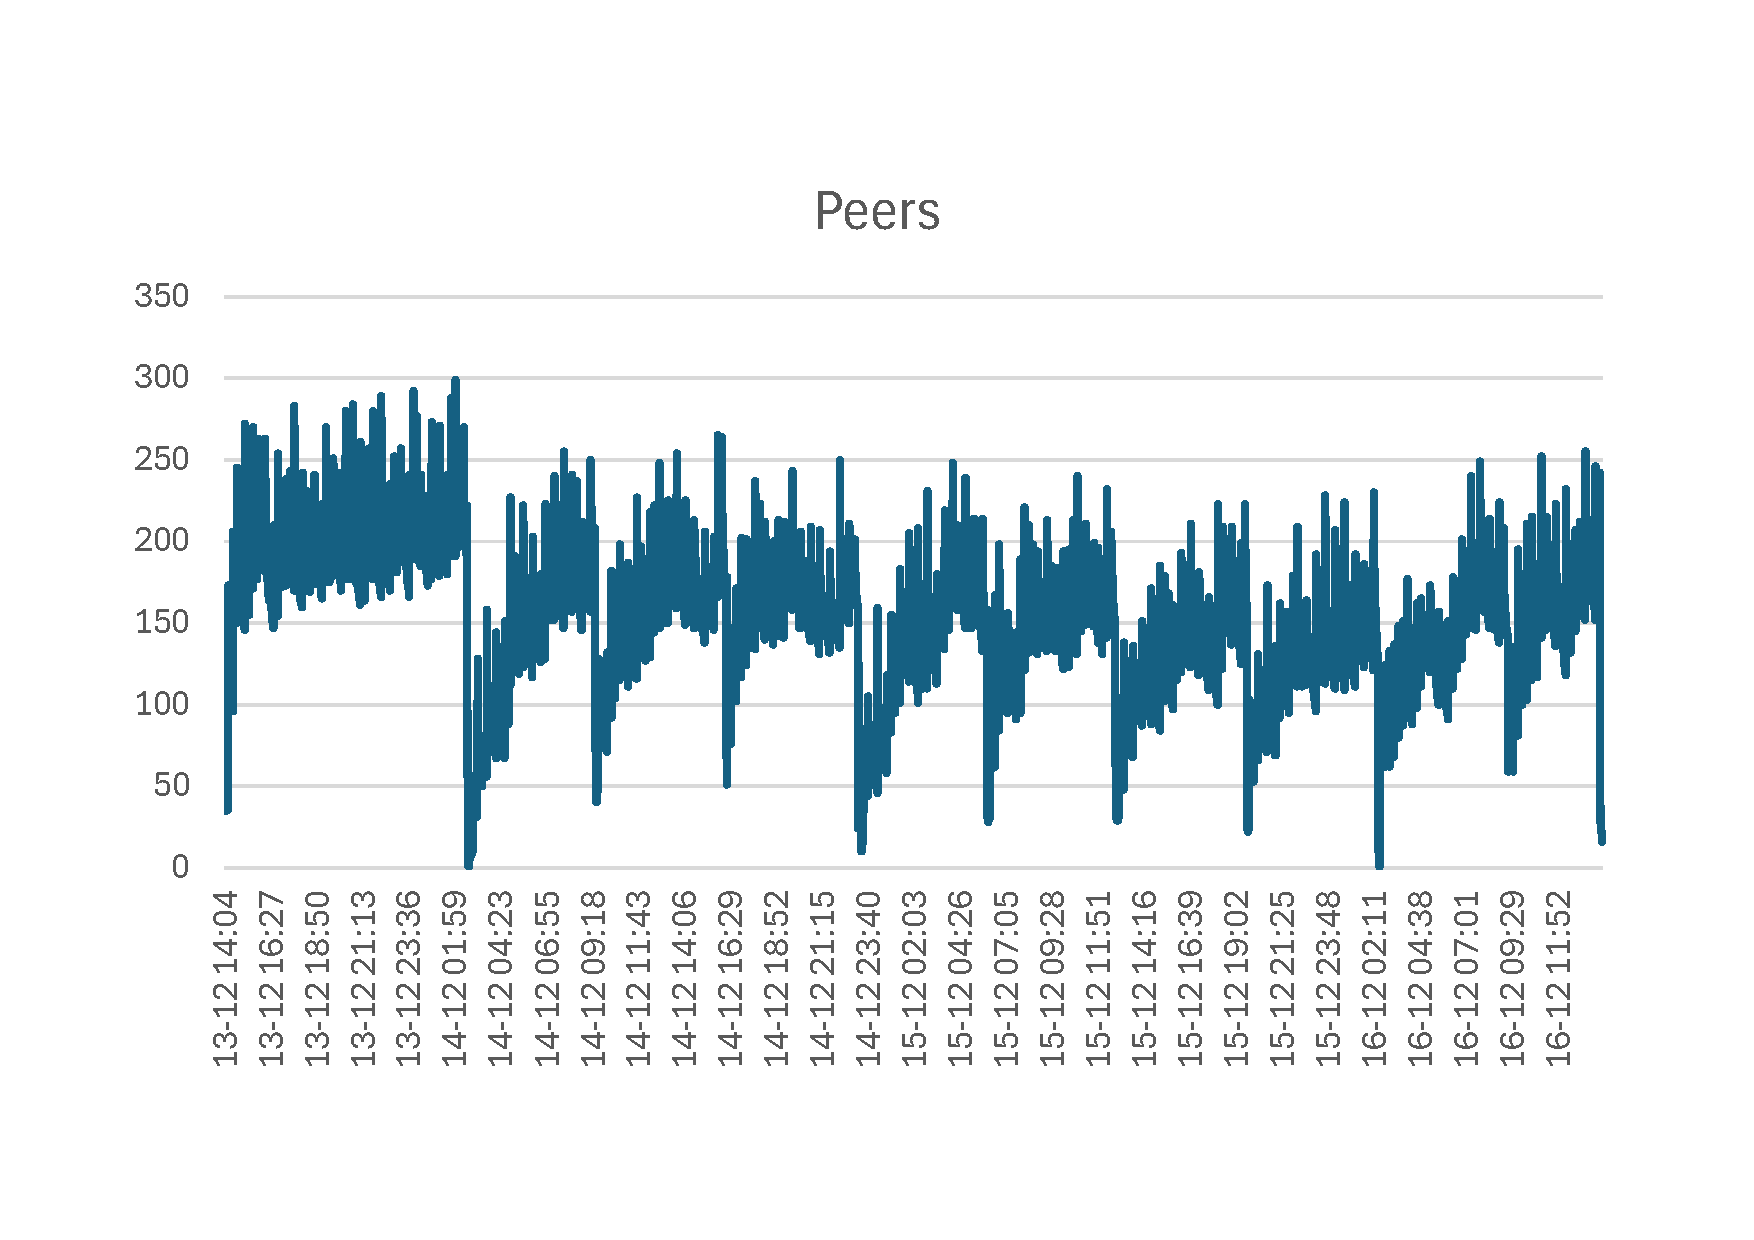
\includegraphics[scale = 0.5]{figures/conPeer2}
    \caption{The number of peers our node was connected to over the time of the experiment.
    Data points are collected every minute and the average amount of peers connected is 148.}
    \label{fig:peersconnected}
\end{figure*}
Throughout the experiment, we kept track of the number of peers our node was connected to.
The number of connected peers is shown in~\autoref{fig:peersconnected}.
Our node was connected to at most 299 peers at once, and the average was 148 peers.
The number of connected peers fluctuated widely throughout the experiment but continually rose for the first 12 hours.
Then, it would heavily drop and rise again.
This pattern would repeat, but after the first drop, it drops consistently every 7 hours.

\subsection{De-anonymization}\label{subsec:de-anonymization}
During the attack, we discovered a total of 1,195 unique peers.
The results of the de-anonymization attack are shown in~\autoref{tab:distribution}.
The table showcases the distribution of peers into four categories based on the heuristic described in~\autoref{subsec:inspirational-papers}.
Here, we see that 38.661\% of the peers we have encountered have had at least one validator that has been de-anonymized, meaning that the conditions from~\autoref{subsec:inspirational-papers} are fulfilled.
We also see that 5.941\% of the peers we discovered are subscribed to all 64 subnets.
We did not find validators on 35.314\% of the peers we discovered, meaning that we did not receive a single non-backbone attestation from any validator on these peers.
Lastly, we discovered that 20.084\% of peers did not fit into the other categories.
Failing to categorize a peer could be because the peer could be hosting a validator, but we could not, with enough confidence, say that to be the case based on our heuristic.


\begin{table}[]
    \centering
    \caption{Distribution of nodes into the four different categories}
    \begin{tabular}{lll}
        \hline
        & \textbf{Nodes} & \textbf{Distribution} \\ \hline
        \textbf{Deanonymized validators} & 462            & 38.661\%                 \\
        \textbf{64 subnets}              & 71             & 5.941\%                  \\
        \textbf{No validators}           & 422              & 35.314\%               \\
        \textbf{Rest}                    & 240            & 20.084\%                 \\ \hline
        \\
    \end{tabular}
    \label{tab:distribution}
\end{table}


After the attack, we managed to de-anonymize a total of 492,959 validators corresponding to 28\% of the total number of validators in the Holesky network\footnote{As of 2024-01-08 seen on \href{https://holesky.beaconcha.in/}{holesky.beaconcha.in}}.
158,134 of these validators were non-unique, meaning that they had more than one IP address mapped to them over the duration of the attack.
The results are shown in~\autoref{tab:unique vals}.

In total, we logged 1,183 unique IP addresses.


\begin{table}[]
    \centering
    \caption{Number of validators located by our modified Prysm node. The first column indicates the total number of validators. The second column indicates validators with more than one IP-address mapped to it.}
    \begin{tabular}{lll}
        \hline
        & \textbf{Validators} & \textbf{Non-Unique Validators} \\ \hline
        \textbf{Overall} & 492,959             & 158,134                        \\ \hline
        \\
    \end{tabular}
    \label{tab:unique vals}
\end{table}

\subsection{Validator Distribution}\label{subsec:validator-distribution}
\begin{figure*}[!ht]
    \centering
    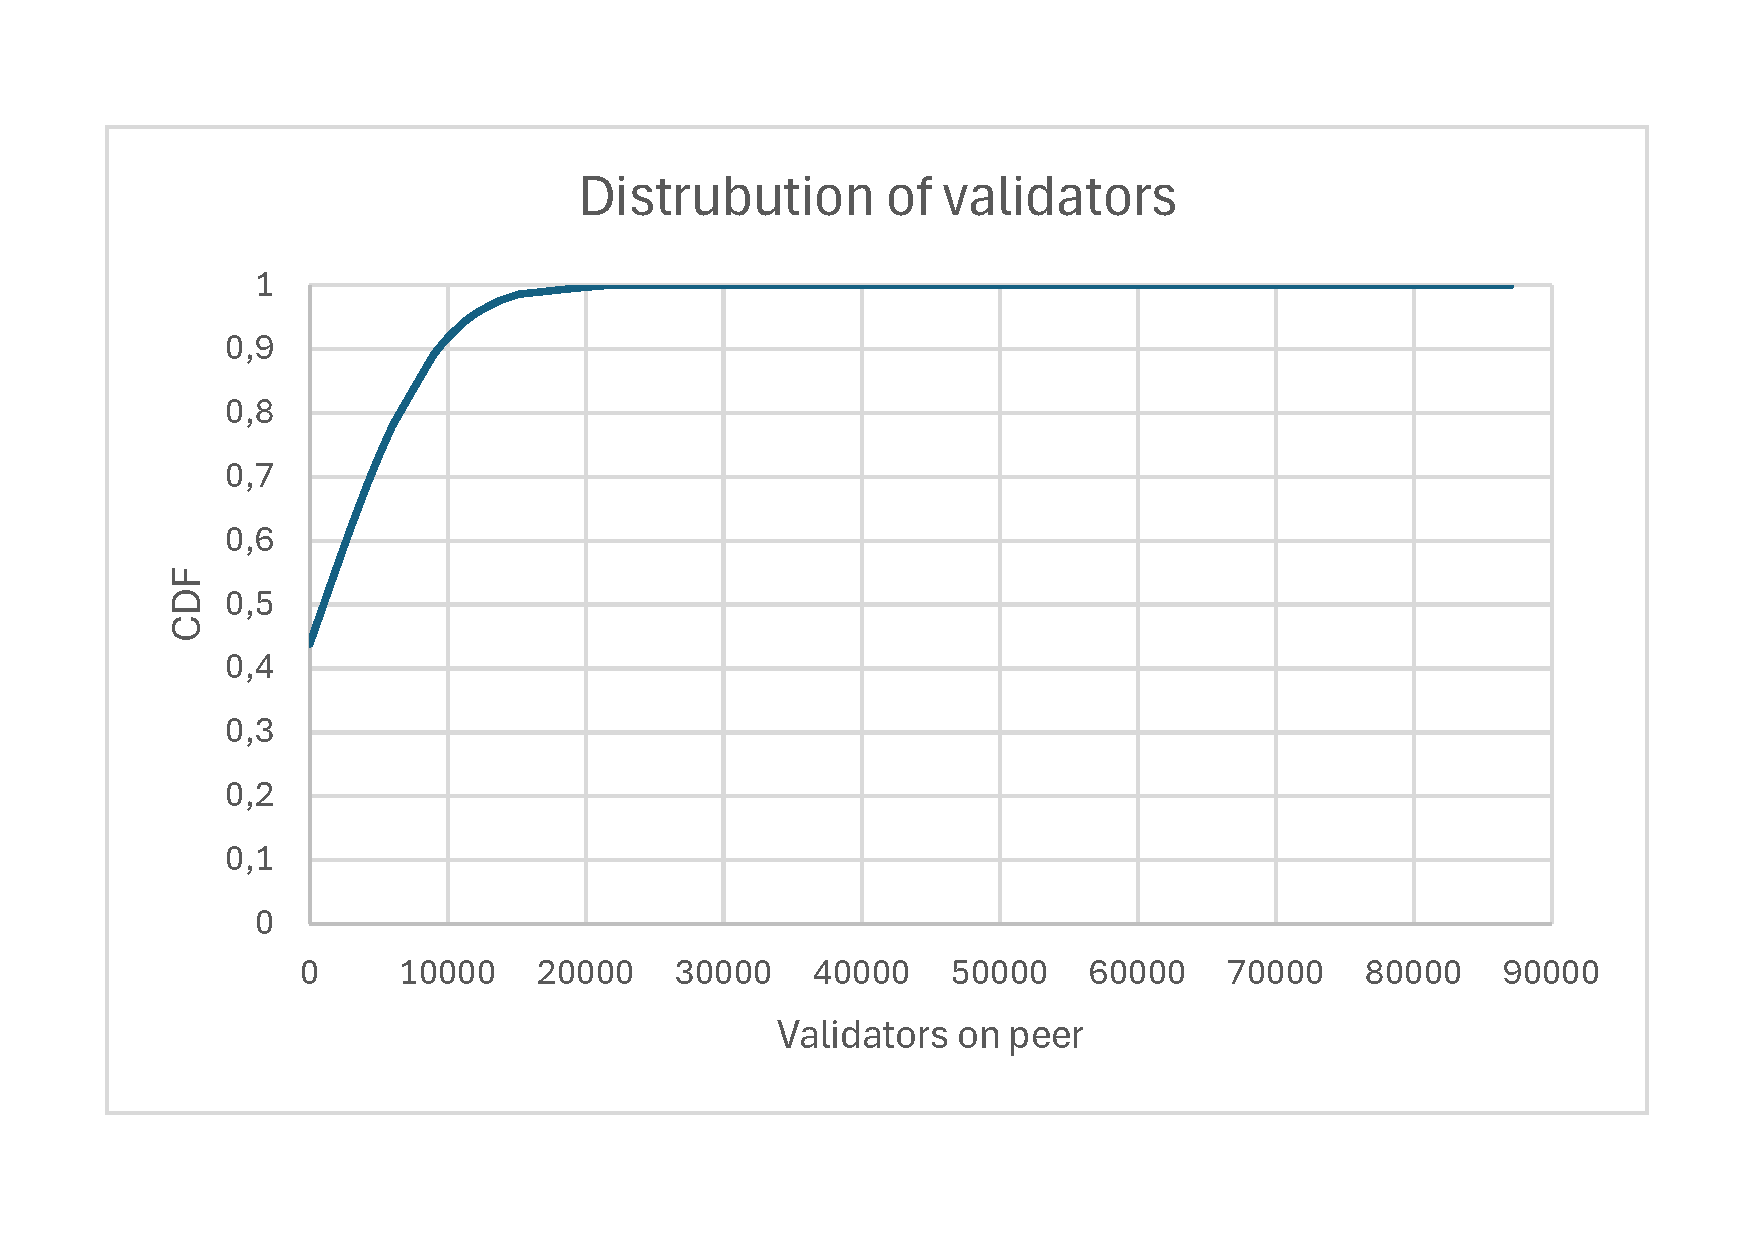
\includegraphics[scale = 0.45]{figures/distval}
    \caption{The cdf showing the distribution of validators on each peer}
    \label{fig:validatorsonpeers}
\end{figure*}
From all the peers we were connected to, we tallied the number of validators on each peer.
The cumulative distribution of validators on each peer is shown in~\autoref{fig:validatorsonpeers}.
Here, we can see that 57\% of the peers we connected to have at least one validator.
The amount of validators on each peer ranges from 0 to 87,028, with the average being 1,003 validators per peer.
We see that the most common number of validators on a peer is 1, with about 7\% of the found peers having only one validator.
We also saw that 110 and 400 were the most common numbers of validators on a peer once we got above 20 validators on a peer.
We found a total of 24 peers that had 10,000 or more validators on them.
    

\section{Discussion}\label{sec:discussion}
This is the discussion
    %! Author = Anders
%! Date = 15-10-2024

\section{Conclusion}\label{sec:conclusion}
This is a potential conclusion section.
    

\section{Future work}\label{sec:future-works}

\subsection{Potential mitigations}\label{subsec:potential-mitigations}
At the moment, there exists an improvement proposal
to include a~\gls{ssle} mechanism, called Whisk, in Ethereum~\cite{EthereumResearchSSLE2024}.

This method aims to improve the security of the network by obfuscating the identity of the proposer.
It does so by making the validators commit to a shared secret which can be bound to a validator's identity and randomized to match the specific validator's identity.

Every epoch a random set of validators are chosen to gather commitments from a set of validators using~\gls{randao}.
Proposers then shuffle the commitments over the duration of 8182 slots.
At the end of that period,~\gls{randao} is then used to map the shuffled list onto the slots in the same way it has been done since Ethereum used~\gls{pos}.
Validators can now decrypt the commitment that matches their identity and propose a block in the slot that they are assigned to.

This whole process is an example of~\gls{zkp} where the point is that every validator is able to prove that it is their turn to propose a block without revealing their identity.
If an attacker would try to fetch the upcoming proposers, he would only retrieve one of these commitments.
Therefore, it makes it harder
for an adversary to perform the Proposer~\gls{dos} attack since the adversary would not know which validator to target.

Though, it does not prevent the data collection part of the attack, which is used to de-anonymize the validators.

But hindering a~\gls{dos} attack in itself is a good reason
to look at implementing~\gls{ssle} in Ethereum as a further step to improving the security of the network.


\subsubsection{More Nodes}\label{subsubsec:more-nodes}
The attack we have performed in this paper is based on the fact that we are able to gather information about the validators in the network by logging attestations.
But since every validator has multiple taske, those being broadcasting and aggregating attestations, and proposing blocks, a possible solution to the attack could be to increase the number of nodes each validator uses.
The validators could then use one node for broadcasting attestations and aggregating attestations, and another node for proposing blocks.
This would make it harder for the attacker to~\gls{dos} the proposer when they have to propose a block since all the attestations that the attacker has gathered would be from a different node with a different IP than the one that is proposing the block.

This would not stop an attacker in de-anonymizing attesters, but it would make it harder for the attacker to perform a~\gls{dos} attack on the validators.
It would however increase the threshold for entry in the system for validators since they would have to run more nodes.

\subsubsection{K-anonymity}\label{subsubsec:k-anonymity}
Another possible solution to the de-anonymization part of the attack could be to implement a k-anonymity system.
Using the Prism Ethereum client, it is possible to choose trusted peers as additional relays for the messages.
This would make at harder to de-anonymize validators as is would make it difficult to match a validator to a fixed IP address.
The group of peers that band together will make up a k-anonymity group.
This would then require the attacker to attack multiple nodes at once when trying to stop a proposer from proposing a block.

This solution would make it harder for the attacker to de-anonymize validators and perform the~\gls{dos} attack.
Though, this would also require new validators in the system to have a set of trusted peers that they can use as relays for their messages.
This would also increase the threshold for entry in the system for validators as well as increase the latency within the system due to the increased number of hops the messages would have to go through.


\subsection{Further research}\label{subsec:further-research}
Due to time constraints, we were not able to fully reproduce the attack mentioned in~\cite{heimbach2024deanonymizingethereumvalidatorsp2p}.
In the original paper, they run their experiment on the mainnet, while we ran our experiment on a testnet.
This means that the results of the two experiments could differ due to the differences in the two networks.
With more time, it would be interesting to run our experiment on the mainnet to see if the results would more closely align with the original paper.


Another place to look for further research would be to implement the~\gls{dos} attack as a follow-up to this paper.
Since this paper mainly focuses on the data collection part of the attack, it would be interesting to see how the~\gls{dos} attack would use the data collected to stop a proposer from proposing a block.
We can see a clear use case for the data collected in the~\gls{dos} attack, and it is clear that this is a possible attack vector that could be used to obstruct the proposer from proposing a block and gain the rewards that come with it.
This however would need to be tested on a local testnet since unlike the data collection part of the attack, the~\gls{dos} attack would have a negative impact on the network and cause a loss of ether for the validators that are being attacked if successful.
    

\section{Acknowledgements}\label{sec:acknowledgements}
We want to express our sincere gratitude to Daniele Dell'Aglio and Michele Albano for their supervision and guidance throughout this thesis.

We also acknowledge the usage of AI tools such as ChatGPT, GitHub Copilot, and Grammarly.
These have been used for clarification and implementation purposes.

    \clearpage
    %\printglossary[type=\acronymtype]

    \printbibliography

    \appendices % You can use \appendix if you only have a single appendix
    %! Author = Runge
%! Date = 29-12-2023

% Main appendix file
% Insert appendix sections below
%! Author = ander
%! Date = 18-10-2024
\section{Attacks on Ethereum}\label{sec:attacks-on-ethereum}
\subsection{Reorg}\label{subsec:reorg}

\subsection{DoS}\label{subsec:dos}
We've found three different kinds of DoS attacks that either were or are possible to perform on Ethereum.

One of the attacks is called \textit{under-priced opcodes}~\cite{10.1145/3391195,9815256}.
This attack works because Ethereum has a gas mechanism to reduce abuse of computing resources.
Though when a contract has a lot of underpriced opcodes, they will consume many resources.
Execution of contracts requires a lot of resources.

To mitigate this,
Ethereum has raised the gas cost of opcodes
to preserve the number of transactions-per-second~\cite{Opcode-mitigation}~\footnote{
\href{https://github.com/ethereum/EIPs/blob/master/EIPS/eip-150.md}{EIPs/EIPS/eip-150.md at master ethereum/EIPs GitHub}}.

Another attack,
which is closely related to the former, is \textit{empty account in the state trie}~\cite{10.1145/3391195,9815256}.
This attack was possible
because the existence of empty accounts increases the transaction processing time and synchronization.
An empty account is an account with zero balance and no code.
The attack required the proposer to select only the transactions of the adversary,
which could be insured by offering a higher gas price.

The mitigation is a combination of the one
explained for \textit{under-priced opcodes} as well as a mitigation
for clearing empty accounts~\cite{Opcode-mitigation,empty-account-mitigation,empty-account-eip-mitigation}~\footnote{
\href{https://github.com/ethereum/EIPs/blob/master/EIPS/eip-161.md}{EIPs/EIPS/eip-161.md at master ethereum/EIPs GitHub}}.

The last example of a DoS attack is called \textit{Proposer DoS}~\cite{EthereumSSLE2024,EthereumAttackDefense2024}.
The background to making this attack possible is
that the consensus mechanism uses a publicly known function for choosing the upcoming block proposers.
The adversary is therefore able to compute this in slight advance of the blockchain, s.t.\ each proposer is now known.
After this, the adversary can map the proposer's IP addresses and overload their connection.
A successful attack would leave a proposer unable to propose their block in time.

To prevent this kind of attack,
Ethereum plans
to use something they call~\gls{ssle} which ensures
that only the selected validator knows that they have been selected~\cite{EthereumSSLE2024,EthereumResearchSSLE2024}.

Specifically, a proposal has been made to use an election protocol called Whisk, which is a type of~\gls{ssle}~\cite{Whisk2024}\footnote{\href{https://github.com/ethresearch/Shuffle_SSLE/tree/master/rust_code/src}{Shuffle\_SSLE/rust\_code/src at master ethresearch/Shuffle\_SSLE GitHub}}\footnote{\href{https://github.com/ethereum/consensus-specs/pull/2800}{[WIP] Introduce consensus code for Whisk (SSLE) by asn-d6 Pull Request \#2800 ethereum/consensus-specs GitHub}}\footnote{\href{https://github.com/dapplion/lighthouse/tree/whisk}{GitHub - dapplion/lighthouse at whisk}}.
It works by each validator submitting a commitment to a secret shared by all validators.
The commitments are shuffled s.t.\ no-one can map commitments to the validators,
but each validator knows what commitment belongs to them.
This shuffle-phase goes on for a day, 256 epochs, before using the shuffled proposer list the following day.
Commitments are chosen at random, and the selected proposer will detect its commitment to know when to propose a block.

The shuffling phase requires validators to occasionally shuffle a subset of candidate proposers.
Using a subset is a measure to reduce computation for the validators, as 256 epochs correspond to 8912 proposers.
The shuffle requires a validator to construct a~\gls{zkp} to confirm that the shuffle was performed correctly.

\subsection{Balancing Attack}\label{subsec:balancing-attack}
For this type, we found two attacks.

The first attack we call \textit{LMD-specific balancing attack}~\cite{10.1145/3560829.3563560}.
This attack exploits the~\gls{lmd} \textit{proposer
boosting} by sending out two competing blocks
but giving half the validators one block before the other and the opposite for the other half.
This would create a fork in the blockchain.

Although no mitigation is mentioned,
it requires $W_p/b+1$ adversarial slots~\footnote{where $W_p$ is the proposer boost weight (fx 100 validators/slot: $W_p=0.7\cdot100=70$)
    and $b$ is the fraction of adversaries in the committee in each slot}.


Another balancing attack has the adversary
exploiting adversarial network delay
and strategic voting by a vanishing fraction of adversarial validators
to stall the protocol indefinitely~\cite{10.1007/978-3-031-18283-9_28}~\footnote{
\href{https://github.com/tse-group/gasper-gossip-attack}{GitHub - tse-group/gasper-gossip-attack}}.

Though this attack does depend on networking assumptions that are highly contrived in practice; those being the attacker having fine-grained control over latencies of individual validators.

\subsection{Finality Attack (Bouncing Attack)}\label{subsec:finality-attack-(bouncing-attack)}
For the Ethereum, there exists attacks called finality attacks, also known as bouncing attacks, which have the purpose of denying the blockchain to finalize its block, halting its functionality.

The first attack is a \textit{double finality} attack~\cite{EthereumAttackDefense2024, 10646904}.
It is theoretically possible for an attacker that wants to risk 34\% of the total staked ether.
Two forks finalize simultaneously, creating a permanent split of the chain.

A way to see a mitigation of this is that it is practically impossible given the current value of 34\% of the total staked ether.
Also, voting on two different chains, called double voting, is a slashable offense in the Ethereum chain, so the adversary would get their staked ETH slashed.


Another finality attack is called \textit{33\% finality attack}~\cite{EthereumAttackDefense2024}.
Here, all adversarial ($\geq33\%$) validators can simply go inactive, meaning that a block cannot get $2/3$ attestations which is required to achieve finality.
Therefore, the blockchain would not be able to go further, as it would not be able to achieve finality.

The mitigation for this is called \textit{the inactivity leak}.
The Ethereum chain penalizes the validators who resist voting or are inactive.
Their ETH gets burned until the majority vote has a 2/3 majority.
This makes the attack impractical for the attacker, as it is costly to have $\geq33\%$ of the total staked ETH and their ETH gets burned as well.

\subsection{Avalanche Attack}\label{subsec:avalanche-attack}

\subsection{Bribery}\label{subsec:bribery}

\subsection{Staircase Attack}\label{subsec:staircase-attack}

\end{document}
